\documentclass{article}
\author{Marcin Gólski \and Piotr Kaszubski}
\title{Decision Analysis report 1 - PROMETHEE I, PROMETHEE II, ELECTRE TRI-B}
\usepackage{array}
\usepackage{geometry}
\geometry{lmargin=35pt, rmargin=35pt}
\usepackage{graphicx}
\graphicspath{ {./figures/} }
\usepackage{multicol}
\begin{document}
\maketitle

\section{Data set}

\begin{enumerate}

    \item What is the domain of the problem about?

    We tackle the problem of determining what video game should be purchased or played

    \item What is the source of the data?

    The games' store pages on Steam and DM's judgement

    \item What is the point of view of the decision maker?

    The decision maker is a person with a limited budget of time and money who has a particular taste in video games. They wish to find out what titles would be the best to sink their resources into.

    \item What is the number of alternatives considered? Were there more of them in the original data set?

    15 alternatives are considered. Originally, there were 8 of them, because one of the author's wishlists contained only 8 games. The decision to include already owned games was a motivated by curiosity, the desire to have more informative results, and the need to have at least 12 alternatives in the data set.

    % TODO: I'm unsure how to interpret "preferences".
    % based on the document from lab1, "evaluations" refers to the values for all criteria (g_i)
    % the same document gives some examples of preference information in MCDA, but I'm, as of yet, unsure
    \item Describe one of the alternatives considered (give its name, evaluations, specify preferences for this alternative)

    Representation of one of the considered alternatives - the game "Nebuchadnezzar"

    \vbox{
        \begin{itemize}
            \item Title: Nebuchadnezzar
            \item Price: 71.99
            \item \% of positive reviews: 81
            \item Total number of reviews:1085
            \item System requirements: 3
            \item Content volume: 5
            \item Gameplay: 8
            \item Audio: 6
            \item Graphics: 6
            \item Position on wishlist: 1
        \end{itemize}
    }


    \item What is the number of criteria considered? Were there more of them in the original data set?

    9 criteria are considered. There were 9 criteria in the original data set as well, since we created it ourselves.

    \item What is the origin of the various criteria?
    (catalog parameter / created by the decision maker - how?)

    \verb|price| - full cost of the game, taken from its Steam store page (given in PLN, for Polish market)

    \verb|positive_reviews_percentage|, \verb|number_of_reviews| - same Steam store page

    \verb|system_requirements| - based on the information given on the Steam store page

    \verb|content_volume|, \verb|gameplay|, \verb|audio|, \verb|graphics| - based on authors' personal judgements

    \verb|position_on_wishlist| - position on one of the author's wishlists.
    \item What are the domains of the individual criteria (discrete / continuous)? Note: in the case of continuous
    domains, specify the range of the criterion's variability, in the case of others: list the values. What is
    the nature (gain / cost) of the individual criteria?

    % I would LOVE to use some fancy lingo to justify this
    % something about "finite granularity" (economics?), or being able to map the price to groszes 1-1 by just *100...
    All criteria are discrete (even \verb|price|).

    \verb|price| - self explanatory. Minimum value in the data set: 0 (for "Path of Exile", a free to play game), maximum value: 249.00 ("ELDEN RING")

    \verb|positive_reviews_percentage| - 0-100 scale.

    \verb|system_requirements|, \verb|content_volume|, \verb|gameplay|, \verb|audio|, \verb|graphics| are all judged on a 1-10 scale.

    \verb|position_on_wishlist| - 1 represents the top of the list (the most desired game). If already owned, set to 0 - this seemed to be a natural representation and it reflects the DM's preference for this title, which must hold, since they decided to purchase it already.


    \item Are all criteria of equal importance (should they have the same ”weights”)? If not, can the relative
    importance of the criteria under consideration be expressed in terms of weights? In this case, estimate
    the weights of each criterion on a scale of 1 to 10. Are there any criteria among the criteria that are
    completely or almost invalid / irrelevant?

    No, the criteria are not of equal importance. Here are the estimated criteria weights:
    \begin{itemize}
        \item \verb|price| 7
        \item \verb|positive_reviews_percentage| 10
        \item \verb|number_of_reviews| 5
        \item \verb|system_requirements| 6
        \item \verb|content_volume| 6
        \item \verb|gameplay| 8
        \item \verb|audio| 3
        \item \verb|graphics| 4
        \item \verb|wishlist_position| 6
    \end{itemize}

    The \verb|audio| and \verb|graphics| criteria are of particularly low importance. The authors do not consider them vital to a good experience, but rather additional means of enhancing it.

    \item Are there dominated alternatives among the considered data set? If so, present all of them (dominating
    and dominated alternative), giving their names and values on the individual criteria.

    Yes, there are 3 dominated alternatives: "Last Epoch" (by "Divinity: Original Sin 2"), Gears Tactics (by "Path of Exile"), and "Superliminal" (dominated by both "Portal 2" and "Terraria")

    \begin{center}
        \begin{tabular}{ m{10em}|m{8em}|m{8em} }
            Criterion & Last Epoch & Divinity: Original Sin 2 \\
            \hline
            \hline
            Price & 161.99 & 161.99 \\
            \% of positive reviews & 84 & 95 \\
            Number of reviews & 15629 & 139068 \\
            System requirements & 7 & 7 \\
            Content volume & 9 & 9 \\
            Gameplay & 9 & 9 \\
            Audio & 6 & 9 \\
            Graphics & 7 & 9 \\
            Wishlist position & 7 & 0 \\
        \end{tabular}
    \end{center}


    \begin{center}
        \begin{tabular}{ m{10em}|m{8em}|m{8em} }
            Criterion & Gears Tactics & Path of Exile \\
            \hline
            \hline
            Price & 142.99 & 0 \\
            \% of positive reviews & 75 & 87 \\
            Number of reviews & 5873 & 197422 \\
            System requirements & 8 & 7 \\
            Content volume & 5 & 11 \\
            Gameplay & 5 & 8 \\
            Audio & 4 & 6 \\
            Graphics & 7 & 7 \\
            Wishlist position & 8 & 0 \\
        \end{tabular}
    \end{center}

    \begin{center}
        \begin{tabular}{ m{10em}|m{6em}|m{6em}|m{6em} }
            Criterion & Superliminal & Portal 2  & Terraria\\
            \hline
            \hline
            Price & 71.99 & 45.99 & 35.99 \\
            \% of positive reviews & 94 & 99 & 97 \\
            Number of reviews & 18197 & 336314 & 880572 \\
            System requirements & 4 & 2 & 2\\
            Content volume & 4 & 4 & 8 \\
            Gameplay & 6 & 7 & 8 \\
            Audio & 3 & 8 & 8 \\
            Graphics & 5 & 6 & 5 \\
            Wishlist position & 5 & 0 & 0 \\
        \end{tabular}
    \end{center}

    \item What should the theoretically best alternative look like in your opinion? Is it a small advantage on
    many criteria, or rather a strong advantage on few (but key) criteria? Which?

    An alternative with strong performances on key criteria would be the most preferred. Especially on \verb|positive_reviews_percentage| and \verb|gameplay|, as that would indicate a game that is easy to enjoy.

    \item Which of the considered alternatives (provide name and values on individual criteria) seems to be the
    best / definitely better than the others? Is it determined by one reason (e.g. definitely the lowest
    price) or rather the overall value of the criteria? Does this alternative still have any weaknesses?

    "Terraria" appears to be a strong candidate for the title of the best alternative.
    It is very cheap for a full-priced video game in 2023, without sacrificing any qualities expected from an established title, while also being the most popular (by a wide margin) and exceptionally well received. It is also very light on system requirements due to its design choices, but it presents them very elegantly, leading to a decent score in graphics and an iconic soundtrack.

    \vbox{
    \begin{itemize}
        \item Title: Terraria
        \item Price: 35.99
        \item \% of positive reviews: 97
        \item Total number of reviews: 880572
        \item System requirements: 2
        \item Content volume: 8
        \item Gameplay: 8
        \item Audio: 8
        \item Graphics: 5
        \item Position on wishlist: 0
    \end{itemize}
    }

    \item Which of the considered alternatives (provide name and values on individual criteria) seems to be the
    worst / definitely worse than the others? Is it determined by one reason (e.g. definitely the highest
    price), or rather the overall value of the criteria? Does this alternative still have any strengths?

    The game "Gears Tactics" seems to be the worst. It is mostly due to being rather weak across the board, and doing particularly poorly on the cost type criteria (\verb|price| and \verb|system_requirements|).
    The one redeeming quality are its comparatively good graphics.

    \vbox{
    \begin{itemize}
        \item Title: Gears Tactics
        \item Price: 142.99
        \item \% of positive reviews: 75
        \item Total number of reviews: 5873
        \item System requirements: 8
        \item Content volume: 5
        \item Gameplay: 5
        \item Audio: 4
        \item Graphics: 7
        \item Position on wishlist: 8
    \end{itemize}
    }



\end{enumerate}

% ==================

\clearpage

\section{Problem analysis with the use of PROMETHEE I and II}

\begin{enumerate}

    \item Write the preferential information you provided at the input of the method.

    Raw data available in \verb|./data/games_criteria.csv|

    \begin{center}
    \begin{tabular}{l|c|m{6em}|m{6em}|l}
    Criterion & Type & Indifference threshold & Preference threshold & Weight \\
    \hline
    \hline
    Price & cost & 10 & 20 & 7 \\
    \% of positive reviews & gain & 5 & 10 & 10 \\
    Number of reviews & gain & 100 & 10000 & 5 \\
    System requirements & cost & 1 & 3 & 6 \\
    Content volume & gain & 1 & 4 & 6 \\
    Gameplay & gain & 2 & 5 & 8 \\
    Audio & gain & 3 & 7 & 3 \\
    Graphics & gain & 2 & 5 & 4 \\
    Position on wishlist & cost & 0 & 3 & 6 \\

    \end{tabular}
    \end{center}

    \item Enter the final result obtained with the method. Usually, the first result is not the final one, you can
    slightly adjust the parameter values to your preferences.

    % TODO: why, by the gods, is it not centered?
    % I know it is not ordered in any meaningful way, but that's what I got and I didn't feel that reordering everything would be worth the effort

    \begin{center}
    \begin{table}[!ht]
        \begin{tabular}{c|c|c|c|c|c|c|c|c|c|c|c|c|c|c|c}
            ~ & GT & FTL & DOS2 & T & N & BTD 6 & BiY & LE & SL & GD & RL 2 & P2 & ER & PoE & StS \\
            \hline
            \hline
            Gears Tactics & ~ & ~ & ~ & ~ & ~ & ~ & ~ & ~ & ~ & ~ & ~ & ~ & ~ & ~ & ~ \\ \hline
            FTL Faster Than Light & P & ~ & ? & ~ & P & ~ & ~ & P & P & ~ & P & ~ & P & ? & ~ \\ \hline
            Divinity Original Sin 2 & P & ? & ~ & ~ & P & ~ & ? & P & P & ~ & P & ~ & P & ~ & ? \\ \hline
            Terraria & P & P & P & ~ & P & P & P & P & P & P & P & P & P & P & P \\ \hline
            Nebuchadnezzar & P & ~ & ~ & ~ & ~ & ~ & ~ & P & ~ & ~ & ? & ~ & ~ & ~ & ~ \\ \hline
            Bloons TD 6 & P & P & P & ~ & P & ~ & P & P & P & ? & P & ~ & P & ? & ? \\ \hline
            Baba Is You & P & P & ? & ~ & P & ~ & ~ & P & P & ? & P & ~ & P & ? & ~ \\ \hline
            Last Epoch & P & ~ & ~ & ~ & ~ & ~ & ~ & ~ & ~ & ~ & ? & ~ & ~ & ~ & ~ \\ \hline
            Superliminal & P & ~ & ~ & ~ & P & ~ & ~ & P & ~ & ~ & P & ~ & ~ & ~ & ~ \\ \hline
            Geometry Dash & P & P & P & ~ & P & ? & ? & P & P & ~ & P & ? & P & ? & ? \\ \hline
            Rogue Legacy 2 & P & ~ & ~ & ~ & ? & ~ & ~ & ? & ~ & ~ & ~ & ~ & ~ & ~ & ~ \\ \hline
            Portal 2 & P & P & P & ~ & P & P & P & P & P & ? & P & ~ & P & ? & P \\ \hline
            ELDEN RING & P & ~ & ~ & ~ & P & ~ & ~ & P & P & ~ & P & ~ & ~ & ~ & ~ \\ \hline
            Path of Exile & P & ? & P & ~ & P & ? & ? & P & P & ? & P & ? & P & ~ & ? \\ \hline
            Slay the Spire & P & P & ? & ~ & P & ? & P & P & P & ? & P & ~ & P & ? & ~ \\
        \end{tabular}
    \end{table}
    \end{center}



    \item Compare the complete and partial ranking.

        \begin{tabular}{cb{0.5\linewidth}}
            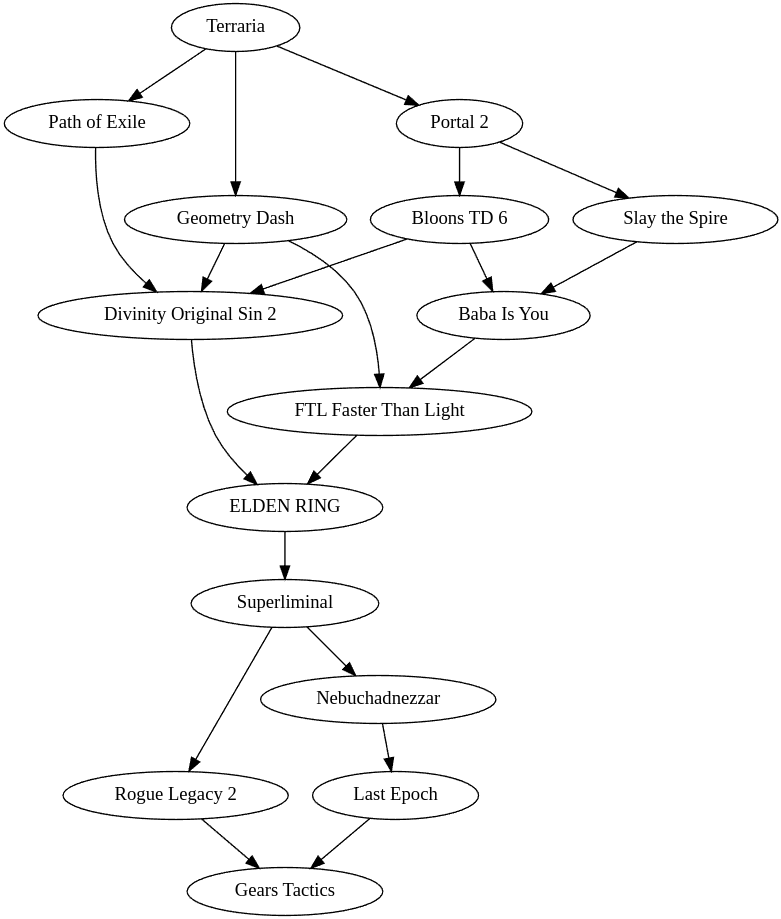
\includegraphics[width=0.5\linewidth]{./figures/p1_partial.png} & \begin{enumerate}
             \item [1.] Terraria
             \item [2.] Portal 2
             \item [3.] Geometry Dash
             \item [4.] Path of Exile
             \item [5.] Bloons TD 6
             \item [6.] Slay the Spire
             \item [7.] Baba Is You
             \item [8.] FTL Faster Than Light
             \item [9.] Divinity Original Sin 2
             \item [10.] ELDEN RING
             \item [11.] Superliminal
             \item [12.] Rogue Legacy 2
             \item [13.] Nebuchadnezzar
             \item [14.] Last Epoch
             \item [15.] Gears Tactics
            \end{enumerate}
        \end{tabular}

        They correspond well to each other, as expected. The complete ranking doesn't capture the full complexity of the relationships, but it gives a faithful "summary" of the results.

    \item Comment on the compliance of the results with your expectations and preferences. Refer, among
    others, to to the results for the alternatives that you indicated as the best and worst during the data
    analysis. What operations were required to obtain the final result (e.g. changing the ranking of criteria,
    adding blank cards, changing the value of threshold)?

    The results mostly comply with the expectations.
    All 4 initial pairwise comparisons are satisfied. Personally, I'm surprised by the good performance of "Geometry Dash".
    "Terraria" and "Gears Tactics" were good picks for the extreme alternatives - they clearly performed best and worst, respectively.
    There were few changes to the criteria were made during the process. The thresholds for price were adjusted seeing how poorly some more expensive games were performing despite their other merits. The authors had disagreements about the ratings of particular games, those were the parameters that took the longest to settle down on.

    \end{enumerate}

% ==================

\clearpage
\section{Problem analysis with the use of ELECTRE TRI-B}

\begin{enumerate}

    \item Write the preferential information you provided at the input of the method.

    Raw data loaded from \verb|./data/games_criteria.csv|, with weights updated
    using the SRF method with the following card stack:
    \begin{itemize}
        \item \% of positive reviews
        \item Gameplay
        \item ---
        \item Content volume
        \item ---
        \item ---
        \item Number of reviews
        \item wishlist\_position
        \item ---
        \item System requirements
        \item Graphics
        \item ---
        \item ---
        \item Price
        \item ---
        \item Audio
    \end{itemize}
    \begin{center}
        \begin{tabular}{l|c|m{6em}|m{6em}|m{6em}|l}
            Criterion & Type & Indifference threshold & Preference threshold & Veto & Weight \\
            \hline
            \hline
            Price & cost & 10 & 20 & 50 & 0.045886 \\
            \% of positive reviews & gain & 5 & 10 & 40 & 0.189873 \\
            Number of reviews & gain & 100 & 10000 & 100000 & 0.123418 \\
            System requirements & cost & 1 & 3 & 7 & 0.09019 \\
            Content volume & gain & 1 & 4 & 6 & 0.156646 \\
            Gameplay & gain & 2 & 5 & 7 & 0.178797 \\
            Audio & gain & 3 & 7 & -- & 0.023734 \\
            Graphics & gain & 2 & 5 & -- & 0.079114 \\
            Position on wishlist & cost & 3 & 7 & -- & 0.023734 \\
        \end{tabular}
    \end{center}


    There are 4 decision classes: Bottom, Mid, High and Top Tiers.

    \item Enter the final result obtained with the method. Usually, the first result is not the final one, you can
    slightly adjust the parameter values to your preferences.

    \begin{tabular}{m{0.5\linewidth}m{0.5\linewidth}}
        \subsection*{Pessimistic Assignment, $\lambda = 0.65$}
        \begin{enumerate}
            \item Top Tier
                \begin{itemize}
                    \item FTL Faster Than Light
                    \item Baba Is You
                    \item Bloons TD 6
                    \item Geometry Dash
                    \item Nebuchadnezzar
                    \item Path of Exile
                    \item Slay the Spire
                    \item Terraria
                    \item Superliminal
                    \item Portal 2
                \end{itemize}
            \item High Tier
                \begin{itemize}
                    \item Rogue Legacy 2
                    \item Gears Tactics
                \end{itemize}
            \item Mid Tier
                \begin{itemize}
                    \item Divinity Original Sin 2
                    \item Last Epoch
                \end{itemize}
            \item Bottom Tier
                \begin{itemize}
                    \item ELDEN RING
                \end{itemize}
        \end{enumerate} &
        \subsection*{Optimistic Assignment, $\lambda = 0.65$}
        \begin{enumerate}
            \item Top Tier
                \begin{itemize}
                    \item FTL Faster Than Light
                    \item Baba Is You
                    \item Bloons TD 6
                    \item Geometry Dash
                    \item Nebuchadnezzar
                    \item Path of Exile
                    \item Slay the Spire
                    \item Terraria
                    \item Superliminal
                    \item Portal 2
                    \item Rogue Legacy 2
                    \item Divinity Original Sin 2
                    \item Last Epoch
                    \item ELDEN RING
                \end{itemize}
            \item High Tier
                \begin{itemize}
                    \item Gears Tactics
                \end{itemize}
            \item Mid Tier
                \begin{itemize}
                    \item <empty>
                \end{itemize}
            \item Bottom Tier
                \begin{itemize}
                    \item <empty>
                \end{itemize}
        \end{enumerate}
    \end{tabular}



    \item Comment on the compliance of the results with your expectations and preferences. Refer, among
    others, to to the results for the alternatives that you indicated as the best and worst during the data
    analysis. What operations were required to obtain the final result (e.g. changing the ranking of criteria,
    adding blank cards, changing the value of threshold)?

    Top Tier seems a bit too inflated in both cases. This could be
    mitigated by adjusting the boundary to be less accessible, or adjusting
    the weights (perhaps there is some pattern in the data that makes it
    easy to fit everything into that one particular class).

    The results are relatively pleasing -- especially the pessimistic
    assignment. ELDEN RING sits at rock bottom, probably due to its
    unfavorable price tag. A lot of more accessible games are above it. It
    is a bit surprising that Divinity Original Sin 2 is only in the Mid
    Tier, considering its incredibly high values on most criteria, except
    the price.

    We played with the threshold a bit to see if these results could be tweaked, but
    there wasn't much observable difference -- I believe it's due to a lot
    of these assignments being dictated by discordance.

    \item Compare the optimistic and pessimistic class assignments.

    When moving from pessimistic to optimistic metric, most titles get
    moved to the Top Tier. Interestingly, this happens to all alternatives
    below High Tier, yet Gears Tactics stays in High Tier. Perhaps it loses
    major points on one of the criterions, which successfully prevents it
    from being promoted up.

    \item Comment on the compliance of the results with your expectations and preferences. Refer, among
    others, to to the results for the alternatives that you indicated as the best and worst during the data
    analysis. What operations were required to obtain the final result (e.g. changing the ranking of criteria,
    adding blank cards, changing the value of threshold, boundaries or the $\lambda$ parameter)?

    Already answered in 3.

    \item Second iteration of problem solving

    Let's artificially assign low weights to everything except the price, to
simulate a buyer motivated only by their wallet:

\begin{center}
    \begin{tabular}{l|c|m{6em}|m{6em}|m{6em}|l}
        Criterion & Type & Indifference threshold & Preference threshold & Veto & Weight \\
        \hline
        \hline
        Price & cost & 10 & 20 & 50 & 0.84 \\
        \% of positive reviews & gain & 5 & 10 & 40 & 0.02 \\
        Number of reviews & gain & 100 & 10000 & 100000 & 0.02 \\
        System requirements & cost & 1 & 3 & 7 & 0.02 \\
        Content volume & gain & 1 & 4 & 6 & 0.02 \\
        Gameplay & gain & 2 & 5 & 7 & 0.02 \\
        Audio & gain & 3 & 7 & -- & 0.02 \\
        Graphics & gain & 2 & 5 & -- & 0.02 \\
        Position on wishlist & cost & 3 & 7 & -- & 0.02 \\
    \end{tabular}
\end{center}

\newpage
The new grouping presents itself as follows:

\begin{tabular}{m{0.5\linewidth}m{0.5\linewidth}}
    \subsection*{Pessimistic Assignment, $\lambda = 0.65$}
    \begin{enumerate}
        \item Top Tier
            \begin{itemize}
                \item FTL Faster Than Light
                \item Baba Is You
                \item Geometry Dash
                \item Path of Exile
                \item Terraria
                \item Bloons TD 6
                \item Portal 2
            \end{itemize}
        \item High Tier
            \begin{itemize}
                \item Slay the Spire
                \item Superliminal
                \item Nebuchadnezzar
            \end{itemize}
        \item Mid Tier
            \begin{itemize}
                \item Rogue Legacy 2
                \item Divinity Original Sin 2
                \item Last Epoch
                \item Gears Tactics
            \end{itemize}
        \item Bottom Tier
            \begin{itemize}
                \item ELDEN RING
            \end{itemize}
    \end{enumerate} &
    \subsection*{Optimistic Assignment, $\lambda = 0.65$}
    \begin{enumerate}
        \item Top Tier
            \begin{itemize}
                \item FTL Faster Than Light
                \item Divinity Original Sin 2
                \item Baba Is You
                \item ELDEN RING
                \item Last Epoch
                \item Geometry Dash
                \item Path of Exile
                \item Slay the Spire
                \item Terraria
                \item Bloons TD 6
                \item Portal 2
            \end{itemize}
        \item High Tier
            \begin{itemize}
                \item Superliminal
                \item Rogue Legacy 2
                \item Nebuchadnezzar
            \end{itemize}
        \item Mid Tier
            \begin{itemize}
                \item Gears Tactics
            \end{itemize}
        \item Bottom Tier
            \begin{itemize}
                \item <empty>
            \end{itemize}
    \end{enumerate}
\end{tabular}

Now, these results aren't the same as sorting by price, because the veto
thresholds operate independently from the comprehensive concordance index. That
is why we still have some "unintuitive" assignments, like ELDEN RING being in
the Top Tier despite being the most expensive alternative. This only proves that ELECTRE TRI-B is a flexible tool, but at the same time
suffers from having many moving parts, all of which are the responsibility of
the Decision Maker to tweak.

\end{enumerate}

\clearpage
\section{Comparing method results}

PROMETHEE I yielded the most satisfactory results. Its graph representation is intuitive and rich in information. The PROMETHEE methods also reacted very predictably to changes made to criteria and alternatives. The same was not true for ELECTRE - with so many knobs to turn, which were also a bit less obvious from a user's point of view, the changes sometimes brought about unforeseen consequences. This entire experiment demonstrated that the quality of the results greatly depends on DM's understanding of the algorithm itself, which can be problematic.

By the nature of taking on different types of decision problems, the results of the methods are clearly different, but they don't contradict each other. Some alternatives were consistently favoured (Terraria, Path of Exile, Portal 2), while some (Gears Tactics, Last Epoch) did not receive similar praise.

\end{document}